\chapter{Implementation}

% Containing a comprehensive description of the implementation of your software, including the language(s) and platform chosen, problems encountered, any changes made to the design as a result of the implementation, etc.

Agile development processes have been followed throughout the entirety of the project, with the key indicator of progress being working code. As a result, a significant amount of implementation has taken place, with the implementation in its current state beginning to approach a Minimal Viable Product; although there are some key features that have not yet been implemented, that will be the focus in the early stages of the second half of this project. 

\section{Languages and Tools}

Some of the technical decisions regarding language choice are limited by virtue of the architectural decision to build the application using Electron. As a result of this design decision, the primary programming language for the project will be JavaScript. Being able to use JavaScript for both the frontend user interface and the backend service means less context-switching and a more rapid development process. To aid in rapid development of a user interface, a Frontend JavaScript framework will be used. The three primary candidates for the framework choice were React, Vue and Angular. Since I have prior experience with React, and felt that the rate of work would benefit from not having to learn a new framework, React was chosen as the frontend framework for this project, allowing for development using modular, reusable components.

Alongside JavaScript, Electron and React, there are a number of other tools being utilised to aid development. Babel and Webpack are being used to transpile and bundle JavaScript modules, respectively. 

\section{Testing}

In order to ensure that software is of a high quality, significant testing must be carried out. The project will be tested by means of Unit Tests, Functional (End-to-End) tests, and User Acceptance Tests (UAT).

\subsection{Unit Testing}
During the development process so far, unit tests have been written alongside the source code. The tests have been written using the open source test JavaScript framework, Jest. The primary reason why Jest was chosen as the testing framework for this project was due to its Snapshot Testing feature \cite{jest-snapshot}, allowing tests to take a snapshot of a React component's output and then compare all future test runs to this snapshot. This leads to much cleaner test code, which can be written more easily. In addition, the tests for React components use the Enzyme library for manipulating, traversing, and simulating interaction events on the component output \cite{enzyme}. The full unit test suite is run as part of the automated Continuous Integration process, and all tests must pass before feature branches can be merged into the master branch, as regression testing to ensure that new functionality does not cause other tests to fail. A soft target of a minimum of 90\% unit test coverage has been set to increase the likelihood of the tests reliably identifying problems. The master branch currently has unit test coverage of 98.41\%, which is well above the acceptable threshold, and a full coverage report can be found in Appendix \ref{appendix:coverage}.

\subsection{Functional Testing}
In addition to the unit tests described previously, this project will make use of automated Functional (End-to-End) tests in order to ensure that the functional requirements of the system are met. The functional tests will be based on the Functional Specification for this project, as outlined in Section \ref{sec:functional-spec}. Initially, a functional test runner, Spectron, was set up in the project; however, at present there are problems with the test runner, and work is ongoing to identify and resolve the cause of this issue.

\section{Electron Application Architecture}
As discussed previously the application is being built using the Open Source JavaScript Framework, Electron. Electron has two different types of process; the main process, and renderer processes \cite{electron-architecture}. Each renderer process has the ability to optionally display a web page inside a \textit{BrowserWindow}, and every application must have exactly one Main process. 

The initial architectural implementation of the application had two processes: the main process and a single renderer process. The main process is the parent process to all of the renderer processes, and it is the only process that is able to call native GUI APIs \cite{electron-architecture}. This architecture would use the renderer process for displaying the React user interface, and the main process for running the email client services. By keeping the long-running service in a separate process, the performance of the React app would not be hindered. However, further research indicated that this architecture would not be suitable.

The main process houses the UI thread, and therefore it is imperative that it is not blocked with long-running operations to avoid the whole application from freezing until the main process becomes available again \cite{electron-performance}. As a result, the application was re-architected to make use of two renderer processes; one for the react app and one for the email service, in addition to the main process. These two renderer processes are able to communicate with each other using Electron's built in Inter-Process Communication (IPC) methods. Initially, the two renderer processes are unable to directly communicate with each other, and so the main process must first use IPC to send each of the renderer processes the ID of the other, which they can then use for direct message passing. The nature of this communication initialisation is shown by Figure \ref{fig:sequence-ipc}.

\begin{figure}[h!]
\begin{center}
  \begin{tikzpicture}
    \coordinate (a) at (0,0);
    \coordinate (b) at (0,6);
    \coordinate (c) at (5,0);
    \coordinate (d) at (5,6);
    \coordinate (e) at (10,0);
    \coordinate (f) at (10,6);
    \draw [dashed] (a) -- (b)node[pos=1.1,scale=1]{Service Renderer} (c) -- (d)node[pos=1.1,scale=1]{Main}
    (e) -- (f)node[pos=1.1,scale=1]{UI Renderer};
    \draw[{Latex[length=3mm]}-] ($(a)!0.90!(b)$) -- node[below,scale=1,midway]{broadcast-ui-id}($(c)!0.90!(d)$);

    \draw[-{Latex[length=3mm]}] ($(c)!0.70!(d)$) -- node[below,scale=1,midway]{broadcast-service-id}($(e)!0.70!(f)$);

    \draw[{Latex[length=3mm]}-] ($(a)!0.50!(b)$) -- node[below,scale=1,midway]{submit-login-info} ($(e)!0.50!(f)$);

    \draw[-{Latex[length=3mm]}] ($(a)!0.30!(b)$) -- node[below,scale=1,midway]{login-success} ($(e)!0.30!(f)$);

    \draw[-{Latex[length=3mm]}] ($(a)!0.10!(b)$) -- node[below,scale=1,midway]{login-failure} ($(e)!0.10!(f)$);

  \end{tikzpicture}
  \caption{Sequence Diagram showing nature of IPC between Electron processes}
  \label{fig:sequence-ipc}
\end{center}
\end{figure}

\section{Email Sending and Receiving Prototype}
In order to gain an understanding of how best to handle email sending and receiving, a prototype application was built. This gave an opportunity to test different methods in an isolated place. In order to build the prototype as quickly as possible, it used a command line interface (CLI), rather than connecting to the React UI. After building these prototypes, very little work was required to integrate them into the main application, in the form of JavaScript Modules with simplified interfaces.

\subsection{Sending Email}
Emails are to be sent through the Simple Mail Transfer Protocol (SMTP) \cite{smtp-rfc} as this is the recognised standard for sending of email and is supported by all email providers. It was decided early in the implementation process that an existing library should be used to handle email sending, to avoid the complex and time-consuming task of building a client that implements the SMTP protocol from scratch. The SMTP client is responsible for establishing a two-way transmission channel with a SMTP server, and transferring mail messages that server.

Research revealed two JavaScript libraries for creating SMTP clients. These are Nodemailer \cite{nodemailer} and smtp-client \cite{smtp-client}. The smtp-client library works at a relatively low-level, requiring each SMTP command to be manually invoked and sent to the server. It was decided that this low-level of control was not required for this project, and that the higher-level abstraction provided by Nodemailer would be more suitable. Using Nodemailer, sending a message could be done simply using the code as shown in Figure \ref{fig:smtp-code}.

\begin{figure}[h!]
  \centering
    \begin{minted}[frame=single]{js}
      const transporter = nodemailer.createTransport(accountInfo);

      transporter.verify(error => {
        if (error) {
          console.log('There was a problem signing in.');
        }
      });

      const info = await transporter.sendMail({
        from: accountInfo.auth.user,
        to: sendMessageAnswers.to,
        subject: sendMessageAnswers.subject,
        text: sendMessageAnswers.message
      });
    \end{minted}
  \caption{Code for sending a message using Nodemailer}
  \label{fig:smtp-code}
\end{figure}

The result of this prototype was a CLI that could be used to send an email message to an email address with a given subject and body. The CLI output of the application can be seen in Figure \ref{fig:smtp-cli}.

\begin{figure}[h!]
  \centering
  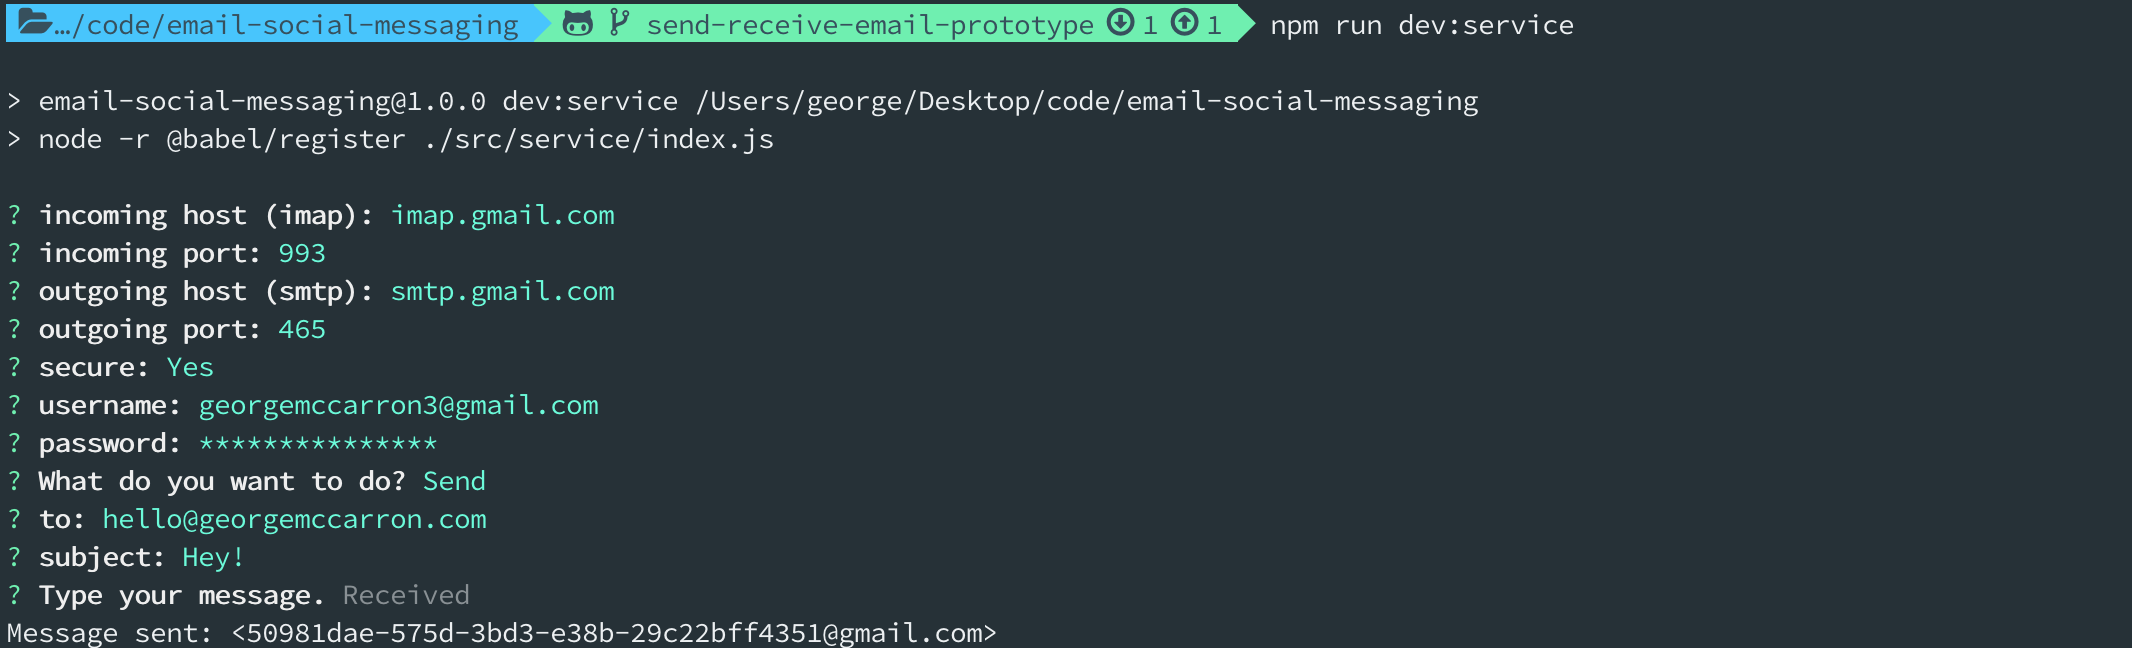
\includegraphics[width=\textwidth]{images/smtp-cli.png}
  \caption{SMTP CLI Prototype Application}
  \label{fig:smtp-cli}
\end{figure}

\subsection{Receiving Email}
After the completion of the SMTP prototype, the prototype application was extended to also allow reading email messages from a remote mailbox. There are two protocols currently in use for accessing messages from mailboxes, IMAP \cite{imap-rfc} and POP3 \cite{pop-rfc}. A key difference between these two protocols is that when a client reads messages using POP3, it downloads the messages, stores them locally, and removes them from the server. With IMAP, the messages are stored permanently on the server (unless explicitly deleted by the client). As a result, it was immediately obvious that IMAP should be used in this project due to the fact that if the software was installed on a different device, all of the users existing conversations should still be accessible.

Preliminary research indicated two suitable libraries for IMAP access in JavaScript. The first of these is node-imap \cite{node-imap} which allows programmatic access to an IMAP server, but works at a relatively low-level, requiring knowledge and manual invocation of the commands used in the IMAP protocol. On the other hand, imap-simple \cite{imap-simple} is a wrapper around the node-imap library which provides a simpler interface. Due to the simplified interface, it was initially decided that imap-simple be used in this project to speed up development time. As development of the prototype progressed, it became apparent that, since imap-simple ``is missing a great deal of functionality from node-imap'' \cite{imap-simple}, it was not going to be possible to use it in this application. 
Specifically, the problem with imap-simple was related to being able to use the \mintinline{js}{onmail} event listener that is invoked when new messages arrive in the mailbox. As a result, the prototype was re-written using node-imap directly, which while more complex, meant that the required functionality could be achieved.

The prototype searched the \mintinline{js}{INBOX} mailbox for any messages with a specific subject, and displayed the body of these. It also displayed the body of any new messages received while the application was running, if they had the given subject line. The output from the prototype can be seen in Figure \ref{fig:imap-cli}.

\begin{figure}[h!]
  \centering
  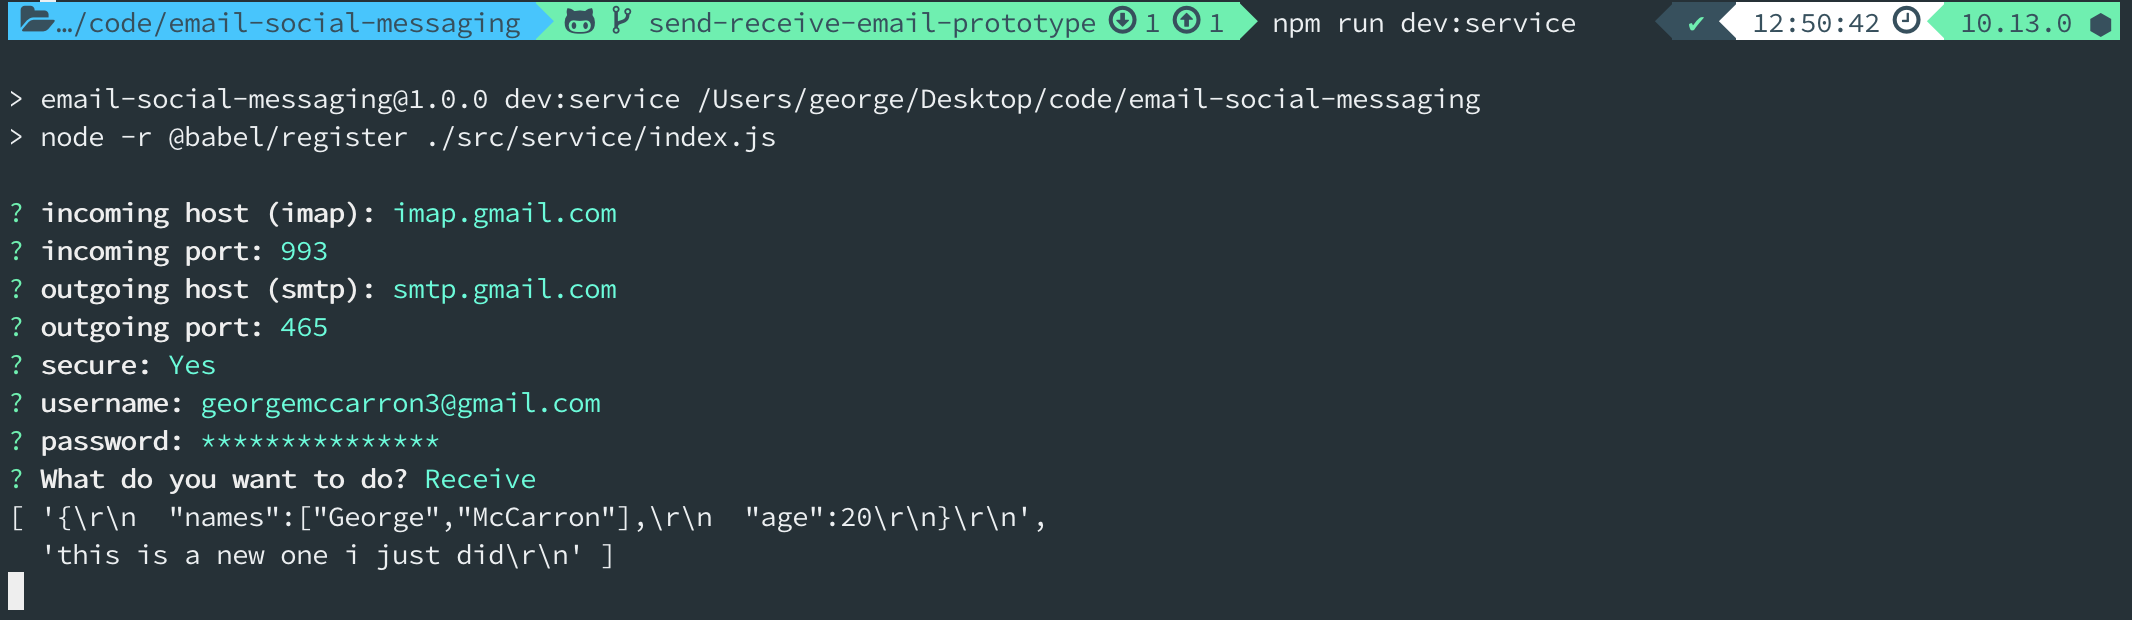
\includegraphics[width=\textwidth]{images/imap-cli.png}
  \caption{IMAP CLI Prototype Application}
  \label{fig:imap-cli}
\end{figure}

\section{User Interface}
As previously discussed, the frontend user interface is built using the React framework. A signifiant amount of implementation work has taken place on the frontend, with the aim of building an interface that can be used in the creation of an MVP. At the present time, most of the user interface elements do not have functionality (i.e. buttons do not invoke any actions) and the interface is hard-coded with sample data, however it serves as a strong starting point for further implementation work. Screenshots of the current user interface implementation, based on the wireframes in Figures \ref{fig:sketch-main} and \ref{fig:sketch-login}, can be seen in Figures \ref{fig:main-ui} and \ref{fig:login-ui}.

\begin{figure}[h!]
  \centering
  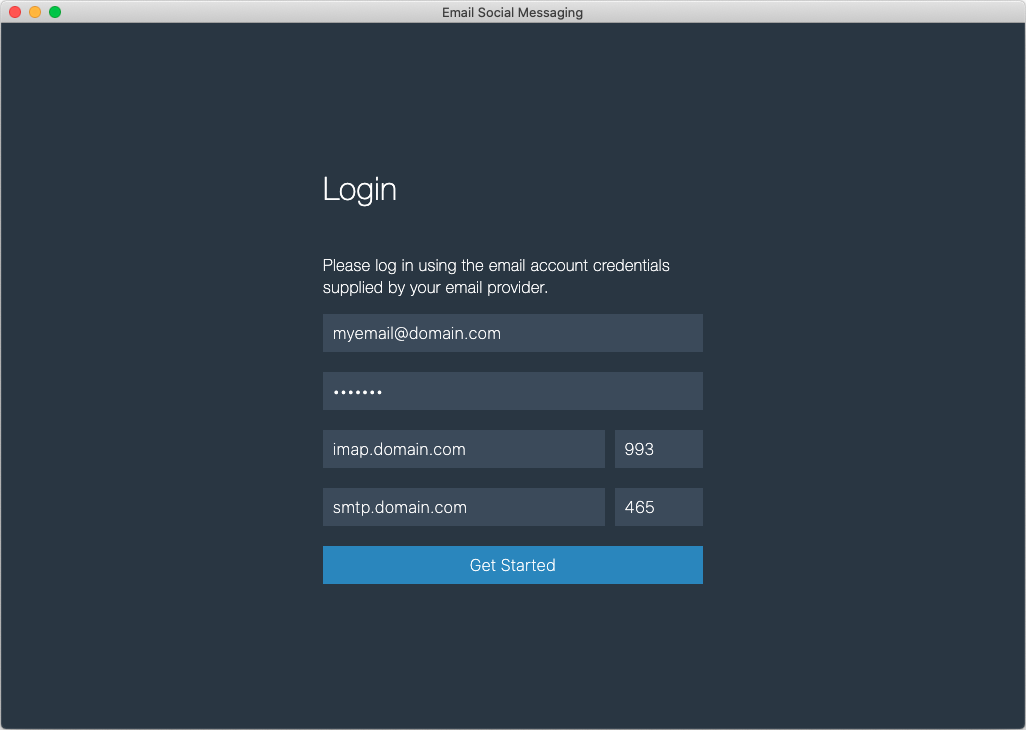
\includegraphics[width=0.8\textwidth]{images/implementation-login.png}
  \caption{Initial Design}
  \label{fig:main-ui}
\end{figure}

\begin{figure}[h!]
  \centering
  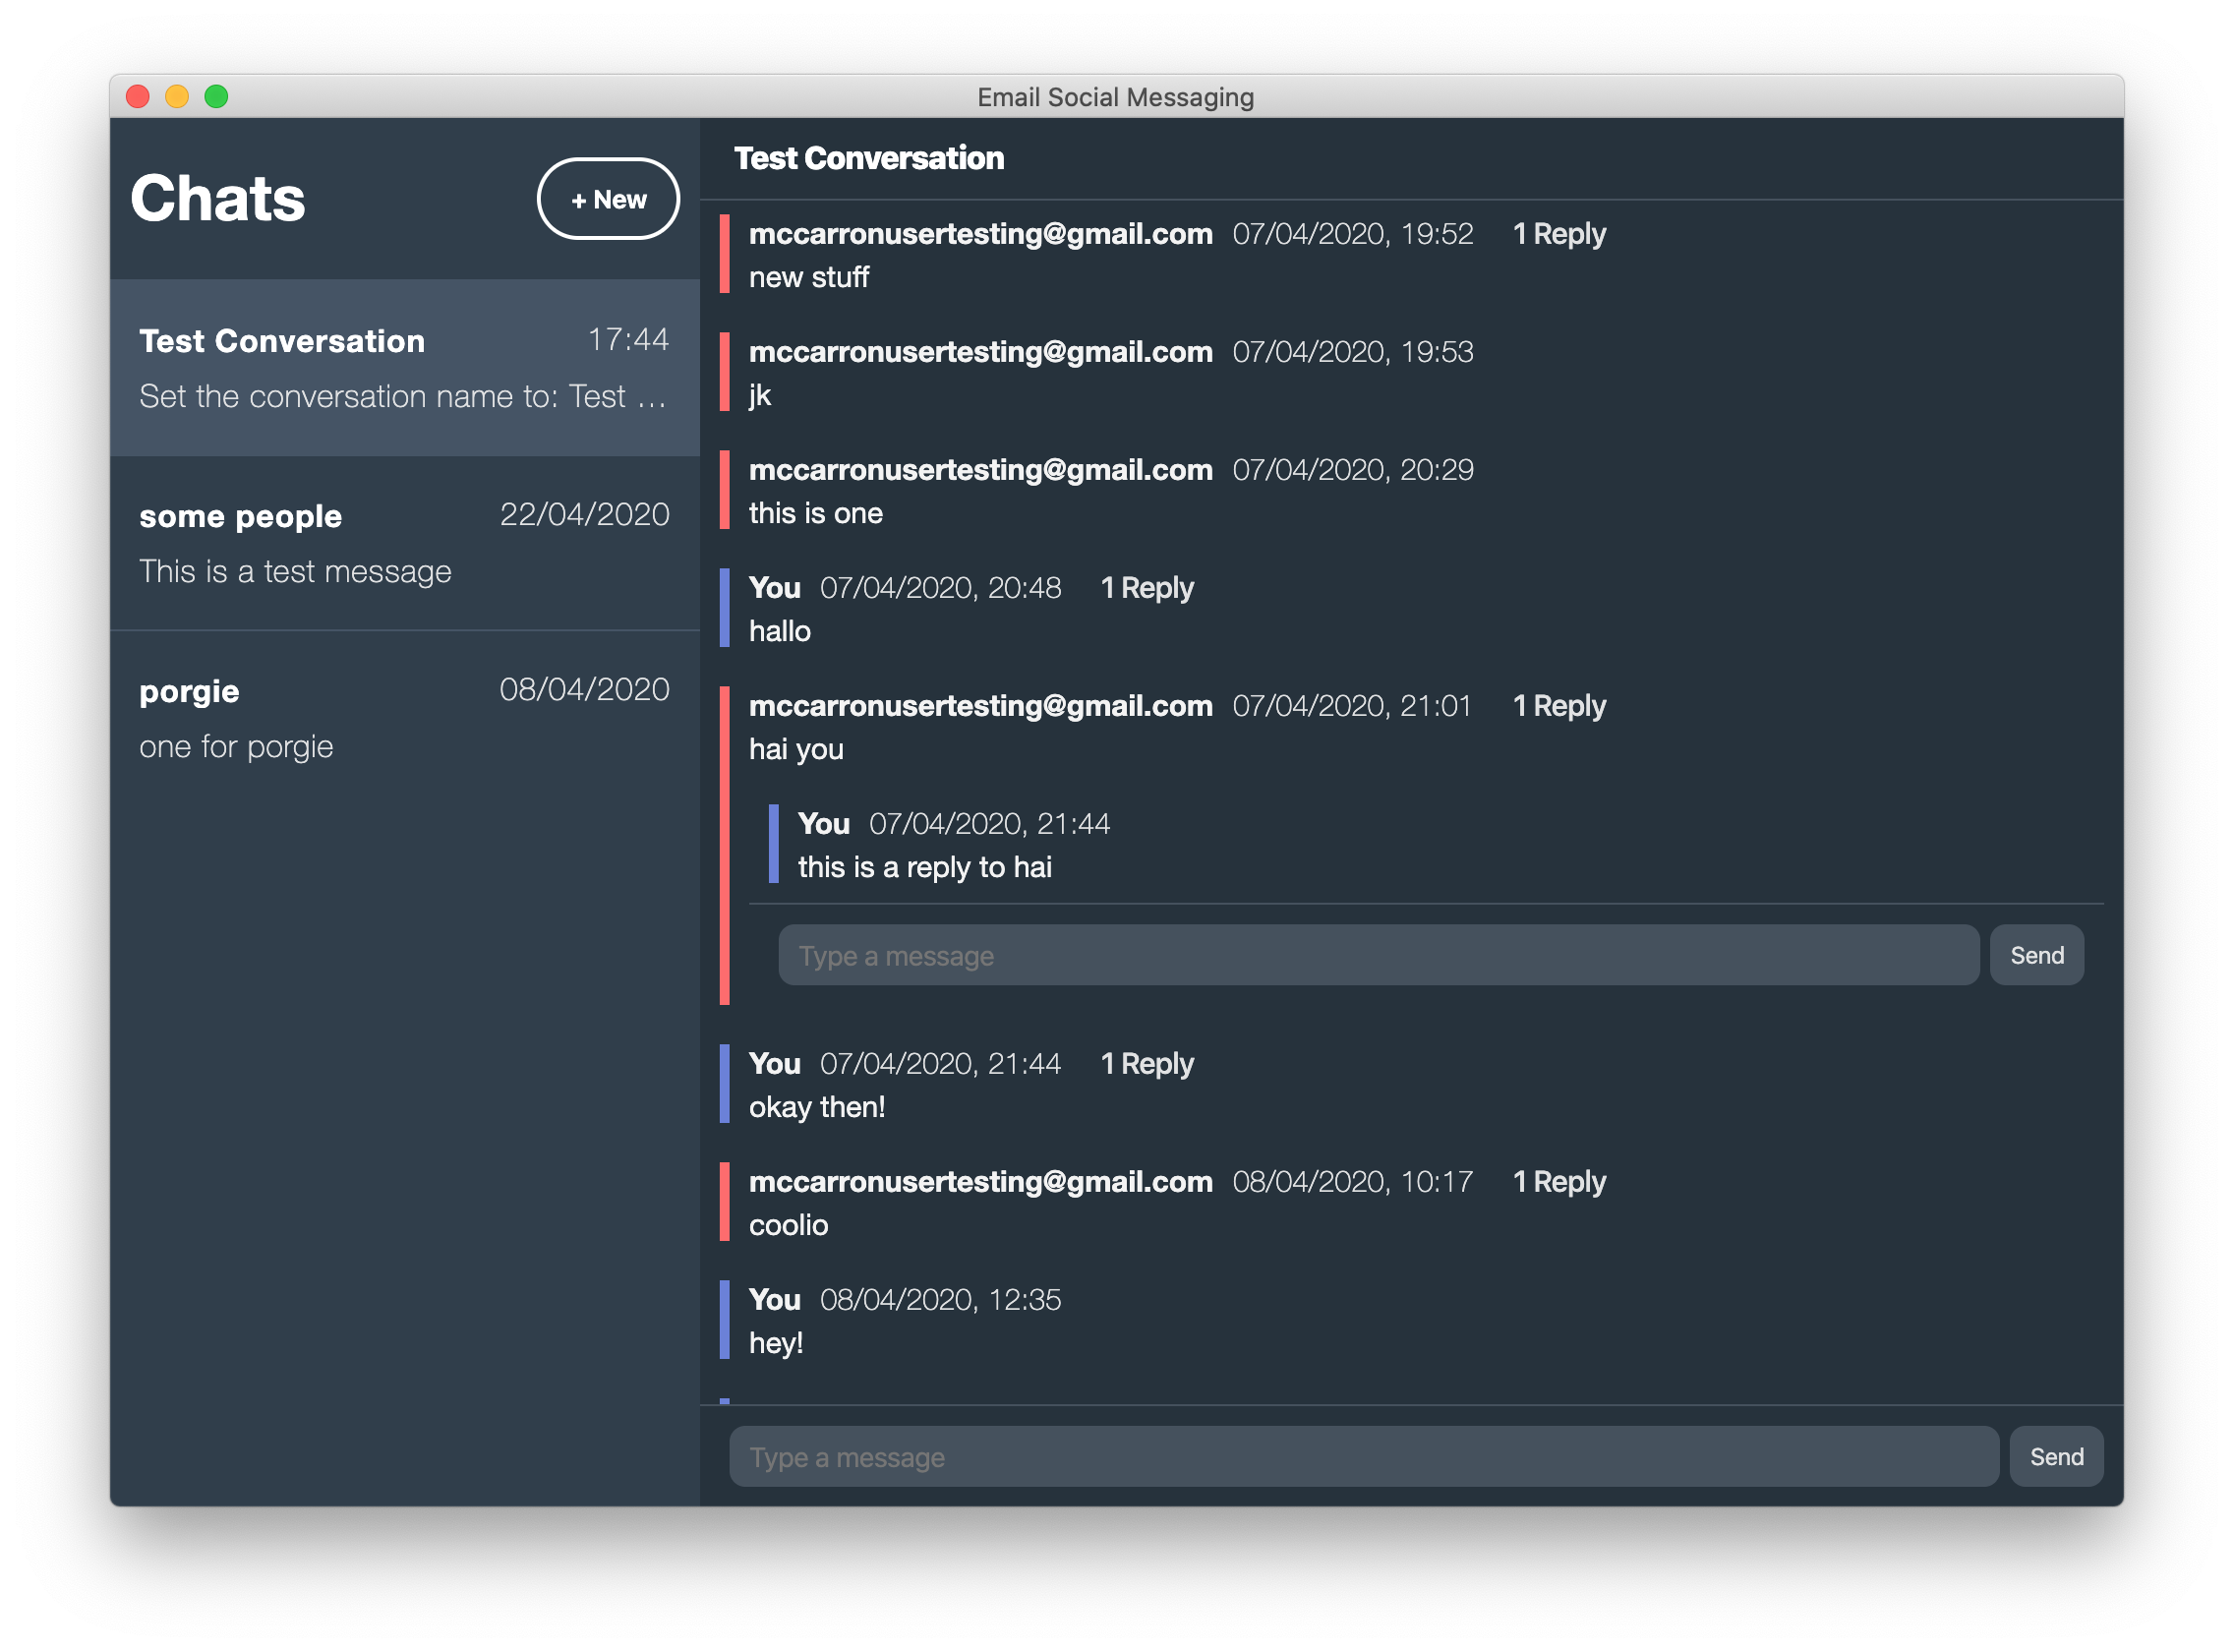
\includegraphics[width=0.8\textwidth]{images/implementation-main.png}
  \caption{Initial Design}
  \label{fig:login-ui}
\end{figure}